\documentclass[a4paper,10pt]{article}
\usepackage[paper=a4paper, hmargin=1.5cm, bottom=1.5cm, top=3.5cm]{geometry}
\usepackage[utf8]{inputenc}
\usepackage[]{algorithm2e}
\usepackage{graphicx}
\usepackage{float}
\usepackage{xcolor}



\begin{document}


\begin{figure}
    
\includegraphics{imagenes/logodc.jpg}
\end{figure}
\begin{figure}[b]
    
\includegraphics[height=7cm]{imagenes/logouba.jpg}
\end{figure}
\begin{center}
    \Huge {Trabajo Práctico II }

\end{center}
\begin{center}
\LARGE{Teoría de las comunicaciones}
\end{center}
\medskip
\medskip
\medskip
\medskip
\medskip
\medskip
\medskip
\medskip
\medskip
\medskip
\medskip
\medskip


\begin{center}
    \begin{tabular}{|c|c|c|}
        \hline
        Integrante & L.U  & Mail \\ \hline  
        Sebastian Taboh & 185/13 & sebi\_282@hotmail.com \\ \hline
        Pedro Mattenet & 428/15 & peter\_matt@hotmail.com \\ \hline
        Gregorio Freidin & 433/15 & gregorio.freidin@gmail.com \\ \hline
        Lucía Romero & 272/15 & luciainesromero@hotmail.com \\ \hline
    \end{tabular}
\end{center}

\newpage

\section{Introducción}
\par{El objetivo de este trabajo práctico es realizar la implementación de una herramienta que imprima el \textit{traceroute} que lleva desde el host local hasta alguna URL o IP pasada por parámetro. Al mismo tiempo también poder mostrar información relevante de cada IP encontrada en el camino, como por ejemplo el RTT promedio o si hay un salto intercontinental de este al router que le sigue.}
\medskip
\medskip
\section{Implementación}
\par{La herramienta fue implementada en Python, utilizando Scapy como biblioteca para el manejo de paquetes.  }
\par{El flujo que diseñamos para llevar a cabo la consigna comenzó creando el \textit{traceroute} con una implementación estándar del mismo. Esta consiste en enviar paquetes con una dirección IP destino igual para todos, pero cada uno con un parámetro TTL distinto (incrementado en uno por cada paquete). De tal manera, se recolectó información sobre cada IP visitada por el paquete para completar su camino al destino original. Para ello se creó dicha herramienta utilizando el siguiente pseudocódigo:}

\medskip
\medskip
\begin{algorithm}[H]
 ttl  = 1 \;
 ultimoRtt = 0\; 
 caminoRecorrido = [ ]\;
 response = responseDeEnviar30PaquetesICMP()\;
    
 \While{respuestasSonDeTipoTimeExceed(response)}{
   caminoRecorrido.Add($\{$\textbf{ip}: response.ip, \textbf{rtt}: response.rttPromedio $-$ ultimoRtt, \textbf{hop\_num}: ttl, \textbf{salto\_inter}: False$\}$)\;
   ttl $+=$ 1\;
   ultimoRtt $=$ response.rttPromedio\;
   response = responseDeEnviar30PaquetesICMP()\;
 
 }
\end{algorithm}


\medskip
\par{Luego, una vez que contábamos con los datos de IPs y RTTs recolectados, nos quedaba aplicar Cimbala para evaluar cuáles de estos saltos tenían un tiempo de respuesta fuera de lo común de la muestra, categorizándolos como saltos intercontinentales.}

\medskip
\par{Al momento de realizar la implementación de la herramienta nos encontramos con diferentes inconvenientes. En primer lugar, no siempre que enviábamos un paquete a una misma dirección, éste tomaba la misma ruta. También sucedía que no todos los routers por los que el paquete viajaba implementaban el protocolo ICMP, por cual, si el paquete vivía su ultimo TTL sobre dicho host, este se perdía.}

\medskip
\par{Para resolver estos problemas decidimos que si al evaluar las respuestas asignadas a la iteración X del traceroute nos llegaban paquetes con varias IPs distintas, nos quedaríamos con la IP más probable, es decir, la que apareciera en mayor cantidad de paquetes \textit{response}.}
\par{Si ningún paquete retornaba, es decir, se perdían todos, decidíamos no asignarle ningún RTT ni IP al salto correspondiente a la iteración X y no tenerlo en cuenta para las diferencias de tiempos entre saltos.}

\medskip
\medskip
\newpage

\section{Experimentación}
\par{La experimentación la realizamos sobre 4 universidades ubicadas en distintos continentes:}
\begin{itemize}
    \item Technische Universität München
    \item Universidad McGill
    \item Universidad del Witwatersrand
    \item Universidad de Chile
\end{itemize}


\medskip
\par{Uno de los inconvenientes con los que nos cruzamos en cada una de las experimentaciones consistió en la facilidad con la cual nuestra implementación del método Cimbala consideraba algunos de los hops de router a router, como outliers. Esto nos llevo a obtener muchos falsos positivos al intentar definir si un salto resultaba intercontinental o no.}
\par{Por ende se realizaron modificaciones en la forma de identificar dichos outliers, las cuales consistieron en utilizar la misma media y desvío en toda iteración del método Cimbala, a diferencia de actualizarlo cada vez que se identificaba un outlier.}

\subsection{Technische Universität München}
\medskip
\par{ Como primer experimento elegimos a la universidad TUM, ubicada en Alemania, de URL \textit{www.TUM.de}. Los resultados obtenidos con nuestra herramienta fueron los siguientes: }

\medskip

\begin{center}
\begin{tabular}{|c | c | c || c | c |}
    \hline
    TTL & Hop & RTT promedio & Contiente & Outlier \\ \hline
1 & 192.168.0.1 & 0.001121& SA &   \\ \hline
2 & 10.36.224.1 & 0.01603& SA &   \\ \hline
3 & 10.242.2.217 & 0.0133& SA &   \\ \hline
4 & 208.178.195.210 & 0.01508& SA &   \\ \hline
5 & 208.178.195.209 & 0.0155& SA &   \\ \hline
6 & 67.17.99.233 & 0.1625& NA & X \\ \hline
7 & * & * & * &  \\ \hline
8 & 4.69.142.209 & 0.2441& EU & X \\ \hline
9 & 195.122.181.62 & 0.2494& EU &   \\ \hline
10 & 188.1.144.38 & 0.2485& EU &   \\ \hline
11 & 188.1.144.133 & 0.2546& EU &   \\ \hline
12 & 188.1.144.254 & 0.261& EU &   \\ \hline
13 & 188.1.37.90 & 0.2616& EU &   \\ \hline
14 & 129.187.0.225 & 0.2625& EU &   \\ \hline
15 & 129.187.255.228 & 0.2621& EU &   \\ \hline
    
  
\end{tabular}
\end{center}
\medskip
\medskip
\medskip

\par{En esta medición podemos ver que el paquete pasa por 3 continentes, marcando correctamente 2 saltos intercontinentales.} 
\par{Ambos saltos marcados como intercontinentales coinciden con la realidad. En un principio las IPs 208.178.195.210 y 208.178.195.209, nos salían que eran de NA, pero averiguando por otras páginas (https://www.iplocation.net/) terminamos definiendo que eran argentinas, lo cual tiene mucho más sentido dados los RTTs obtenidos de cada región.}
\medskip
\par{Resultados:}
\begin{itemize}
    \item  15 de los 16 saltos respondieron el \textit{Time exceeded}
    \item La ruta tiene 2 saltos intercontinentales
    \begin{itemize}
        \item América del Sur - Norte América
        \item Norte América - Europa
    \end{itemize}
    \item Ambos outliers se corresponden con saltos intercontinentales.
\end{itemize}

\medskip
\medskip

\par{A continuación podemos ver graficados los saltos intercontinentales en un mapa, para dar una imagen parcial del recorrido que toman los paquetes al hacer cada consulta: }
\medskip
\begin{figure}[H]
    \centering
    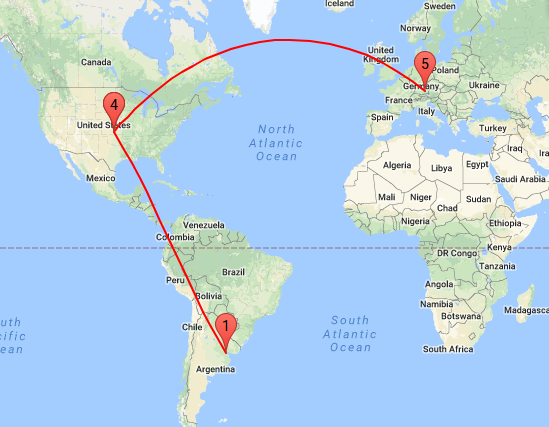
\includegraphics[height=10cm]{imagenes/tracerouteToTUM.png}
    \caption{Trace route www.TUM.de}
\end{figure}


\medskip
\medskip
\par{Utilizando la diferencia entre los RTTs entre un salto y el anterior, luego de normalizarlos calculando los siguientes valores con la ecuación $(X_{i} - \bar{X}) /S $ (donde S es la desviación estándar de los $X_{i}$) se definió el siguiente gráfico. Estos datos también se utilizaron luego para el método Cimbala con el fin de definir cuáles de estos valores cuentan como un outliers, y por ende saltos intercontinentales.}

\medskip
\begin{figure}[H]
    \centering
    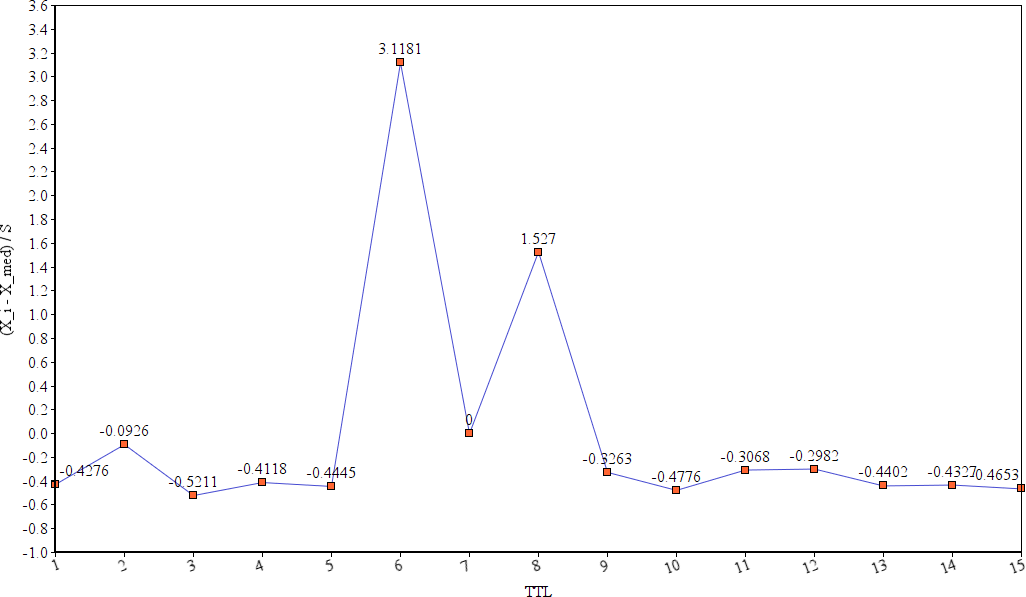
\includegraphics[height=10cm]{imagenes/valorZTUM.png}
    \caption{RTTs por hop (normalizados)}
\end{figure}

\medskip
\par{Se puede notar que los picos de esta función son donde se localizan los saltos intercontinentales, y no se encuentran falsos positivos, ni tampoco positivos que no hayan sido detectados por la experimentación.}



\medskip
\medskip
\medskip


\subsection{Universidad McGill}
\medskip
\par{La segunda medición la realizamos sobre la universidad de McGill ubicada en Canadá, de URL www.mcgil.ca. Y los resultados obtenidos por nuestra herramienta fueron los siguientes: }

\medskip

\begin{center}
\begin{tabular}{|c | c | c || c | c |}
    \hline
    TTL & Hop & RTT promedio & Contiente & Outlier \\ \hline
1 & 192.168.0.1 & 0.0007622& SA &   \\ \hline \\ \hline
2 & 10.36.224.1 & 0.0163& SA &   \\ \hline
3 & 10.242.2.217 & 0.01291& SA &   \\ \hline
4 & 195.22.220.33 & 0.01415& SA &   \\ \hline
5 & 195.22.220.32 & 0.01297& SA &   \\ \hline
6 & 195.22.199.179 & 0.1431& EU (IT) & X \\ \hline
7 & 89.221.41.197 & 0.1459& EU (GER) &   \\ \hline
8 & 89.149.186.130 & 0.1765& NA (USA) &   \\ \hline
9 & 69.31.141.14 & 0.1694& NA (USA) &   \\ \hline
10 & 192.77.63.70 & 0.1704& NA (CA) &   \\ \hline
11 & * & * & * &  \\ \hline
12 & 206.167.128.43 & 0.1704& NA (CA) &   \\ \hline
13 & * & * & * &  \\ \hline
14 & 132.216.255.2 & 0.1784& NA (CA) &   \\ \hline
15 & 132.216.216.166 & 0.2136& NA (CA) &   \\ \hline
16 & 132.216.177.160 & 0.1704& NA (CA) &   \\ \hline
    
  
\end{tabular}
\end{center}

\medskip
\medskip
\medskip

\medskip
\par{Resultados:}
\begin{itemize}
    \item  14 de los 16 saltos respondieron el \textit{Time exceeded}
    \item La ruta tiene 2 saltos intercontinentales
    \begin{itemize}
        \item América del Sur - Europa
        \item Europa - Norte América
    \end{itemize}
    \item Los outliers se corresponden con saltos intercontinentales, pero sin embargo encontramos un falso negativo en el TTL 8, donde vemos que el paquete viaja desde Alemania hacia Estados Unidos, y no figura como outlier.
\end{itemize}

\medskip

\par{A continuación graficamos el recorrido parcial que toman los paquetes dentro de cada request a dicha página: }
\medskip
\begin{figure}[H]
    \centering
    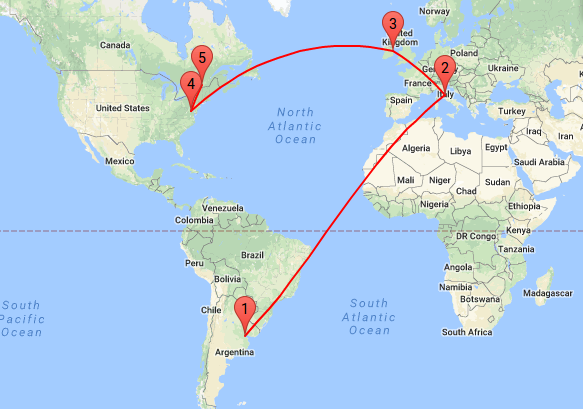
\includegraphics[height=9cm]{imagenes/univesridadCanada.png}
    \caption{Trace route www.mcgill.ca}
\end{figure}


\medskip
\medskip
\par{Por ultimo mostramos los datos utilizados para aplicar Cimbala, o sea los resultados para cada TTL luego de normalizarlos con la ecuación $(X_{i} - \bar{X}) /S $ (donde S equivale la desviación estandar entre los RTTs) para cada $X_{i}$ el valor del RTT promedio en cada uno.}

\medskip
\begin{figure}[H]
    \centering
    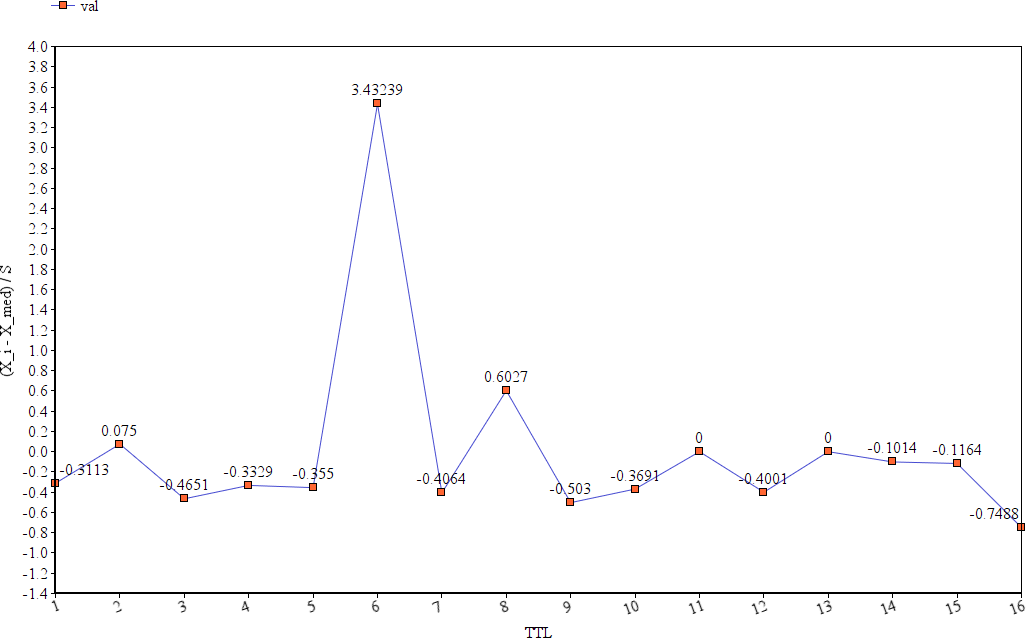
\includegraphics[height=9cm]{imagenes/uniCanada.png}
    \caption{RTTs por hop (normalizados)}
\end{figure}

\medskip
\par{Podemos ver como el salto intercontinental marcado es el máximo local. Y el siguiente salto intercontinental que no fue marcado como outlier es el siguiente que le sigue al  máximo en cuanto a coeficiente de la operación.}



\medskip
\medskip
\medskip

\subsection{Universidad del Witwatersrand}

\medskip
\par{Nuesto tercer experimento lo realizamos ejecutando mediciones sobre la universidad del Witwatersrand ubicada en Australia. Los resultados obtenidos con nuestra herramienta fueron: }

\medskip

\begin{center}
\begin{tabular}{|c | c | c || c | c |}
    \hline
    TTL & Hop & RTT promedio & Contiente & Outlier \\ \hline
1 & 192.168.0.1 & 0.001414& SA(ARG) &   \\ \hline
2 & 10.36.224.1 & 0.01447& SA(ARG) &   \\ \hline
3 & 10.242.2.217 & 0.01391& SA(ARG) &   \\ \hline
4 & 195.22.220.33 & 0.01286& SA(ARG) &   \\ \hline
5 & 195.22.220.32 & 0.01315& SA(ARG) &   \\ \hline
6 & 89.221.35.141 & 0.2027& NA(USA) & X \\ \hline
7 & * & * & * &  \\ \hline
8 & 202.158.194.176 & 0.3522& OC(AU) & X \\ \hline
9 & 113.197.15.146 & 0.3521& OC(AU) &   \\ \hline
10 & 138.44.5.47 & 0.3521& OC(AU) &   \\ \hline
11 & * & * & * &  \\ \hline
12 & * & * & * &  \\ \hline
13 & 129.78.5.11 & 0.3523& OC(AU) &   \\ \hline

\end{tabular}
\end{center}

\medskip
\medskip
\medskip

\medskip
\par{Resultados:}
\begin{itemize}
    \item  10 de los 13 saltos respondieron el \textit{Time exceeded}
    \item La ruta tiene 2 saltos intercontinentales
    \begin{itemize}
        \item América del Sur - Norte América
        \item Norte América - Oceanía
    \end{itemize}
    \item Los outliers se corresponden con saltos intercontinentales. Y no hay falsos positivo ni negativos. En este caso la herramienta funcionó sin ningún problema en cuanto a resulados.
\end{itemize}

\medskip
\par{A continuación graficamos el recorrido parcial que toman los paquetes dentro de cada request a dicha página: }
\medskip
\begin{figure}[H]
    \centering
    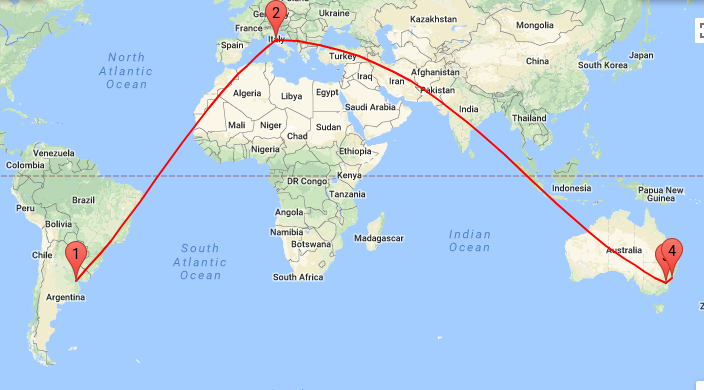
\includegraphics[height=9cm]{imagenes/australiaUni.png}
    \caption{Trace www.sydney.edu.au}
\end{figure}


\medskip
\medskip
\par{Por ultimo mostramos los datos utilizados para aplicar Cimbala, o sea los resultados para cada TTL luego de normalizarlos con la ecuación $(X_{i} - \bar{X}) /S $ (donde S equivale la desviación estandar entre los RTTs) para cada $X_{i}$ el valor del RTT promedio en cada uno.}

\medskip
\begin{figure}[H]
    \centering
    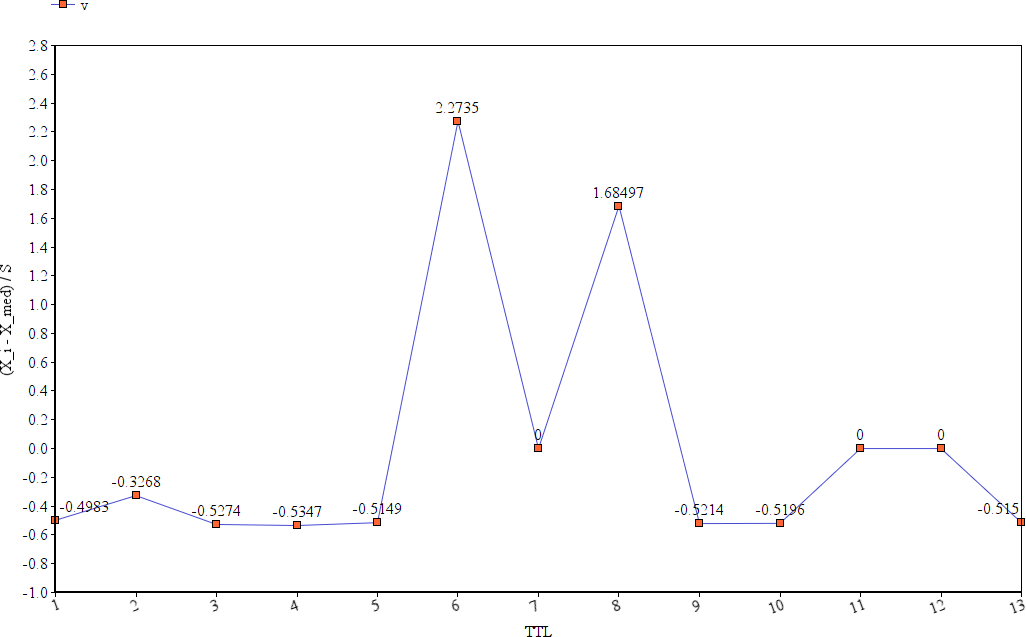
\includegraphics[height=9cm]{imagenes/auUniZVal.png}
    \caption{RTTs por hop (normalizados)}
\end{figure}

\medskip
\par{Podemos ver como los outliers y saltos intercontinentales se corresponden perfectamente con los picos de esta función.}



\medskip
\medskip
\medskip


\subsection{Universidad de Chile}

\medskip
\par{Como último experimento realizamos contra la Universidad de Chile, de URL www.uchile.cl, con el fin de ver que ruta tomaban los paquetes. Terminamos encontrando que  aunque consultemos a una universidad dentro de nuestro mismo continente los paquetes tomaban un camino amplio, desembocando primero en servidores dentro de USA e Italia. Los resultados obtenidos con nuestra herramienta fueron: }

\medskip

\begin{center}
\begin{tabular}{|c | c | c || c | c |}
    \hline
    TTL & Hop & RTT promedio & Contiente & Outlier \\ \hline
1 & 192.168.0.1 & 0.001097& SA(ARG) &   \\ \hline
2 & 10.36.224.1 & 0.01429& SA(ARG) &   \\ \hline
3 & 10.242.2.217 & 0.01278& SA(ARG) &   \\ \hline
4 & 195.22.220.33 & 0.01394& SA(ARG) &   \\ \hline
5 & 195.22.220.32 & 0.01857& SA(ARG) &   \\ \hline
6 & 195.22.219.17 & 0.0416& SA(ARG) &   \\ \hline
7 & 149.3.181.65 & 0.1498& EU(IT) & X \\ \hline
8 & 129.250.2.224 & 0.1462& NA(USA) &   \\ \hline
9 & 129.250.2.111 & 0.145& NA(USA) &   \\ \hline
10 & 129.250.3.208 & 0.1459& NA(USA) &   \\ \hline
11 & 131.103.116.146 & 0.248& NA(USA) & X \\ \hline
12 & 190.208.9.81 & 0.2532& SA(CH) &   \\ \hline
13 & 190.208.9.10 & 0.2554& SA(CH) &   \\ \hline
14 & 200.27.101.242 & 0.2551& SA(CH) &   \\ \hline
15 & 200.89.75.212 & 0.2485& SA(CH) &   \\ \hline
16 & * & * & * &  \\ \hline
17 & 200.89.75.212 & 0.2473& SA(CH) &   \\ \hline
18 & 200.89.76.16 & 0.248& SA(CH) &   \\ \hline


\end{tabular}
\end{center}

\medskip
\medskip
\medskip

\medskip
\par{Resultados:}
\begin{itemize}
    \item  17 de los 18 saltos respondieron el \textit{Time exceeded}
    \item La ruta tiene 3 saltos intercontinentales
    \begin{itemize}
        \item América del Sur - Europa
        \item Europa - Norte América
        \item Norte América - América del Sur
    \end{itemize}
    \item El método para detectar saltos internacionales en este caso no fue muy preciso. Obtuvimos un Positivo correcto que fue el salto desde Argentina a Italia. Pero luego dió falsos negativos desde Italia a USA, y desde USA a Chile. Con un falso positivo dentro de USA, donde hubo un repentino aumento del RTT.
\end{itemize}

\medskip
\par{A continuación graficamos el recorrido parcial que toman los paquetes dentro de cada request a dicha página: }
\medskip
\begin{figure}[H]
    \centering
    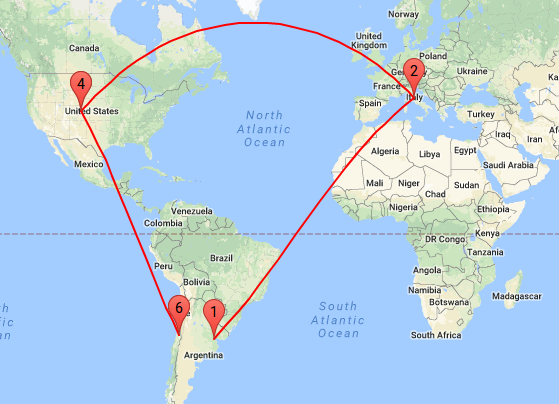
\includegraphics[height=9cm]{imagenes/chileUniChile.png}
    \caption{Trace www.uchile.cl}
\end{figure}


\medskip
\medskip
\par{Luego entonces graficamos los datos obtenidos estandarizados, calculando con la ecuación $(X_{i} - \bar{X}) /S $ (donde S equivale la desviación estándar entre los RTTs). Estos son los resultados utilizados para aplicar Cimbala, y asi entonces poder definir cuales efectivamente cuentan como outliers.}

\medskip
\begin{figure}[H]
    \centering
    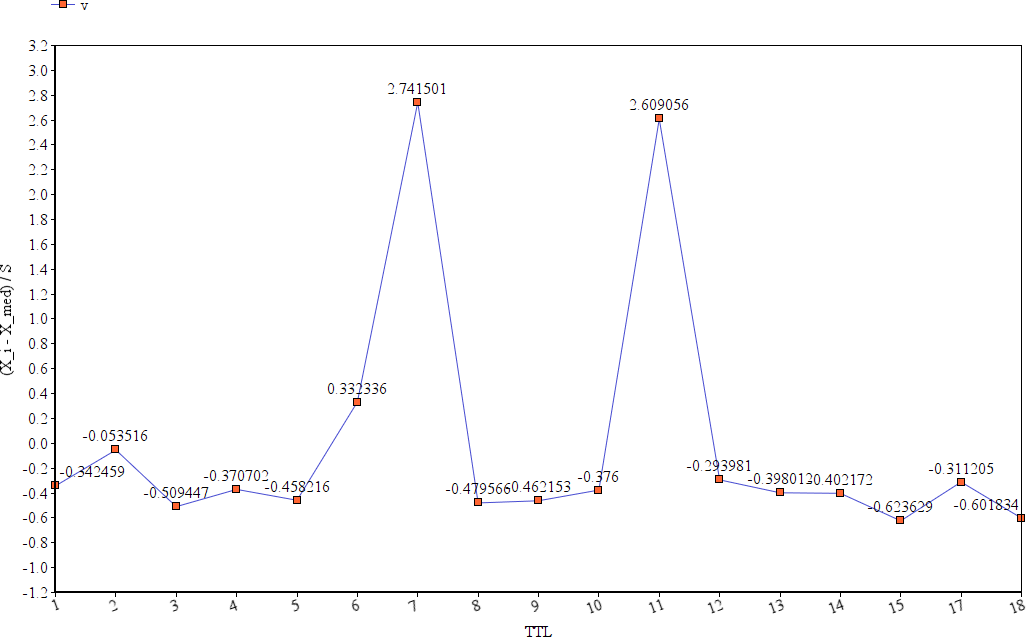
\includegraphics[height=9cm]{imagenes/uCHileZ.png}
    \caption{RTTs por hop (normalizados)}
\end{figure}

\medskip
\par{Podemos ver como los outliers se corresponden con los picos de la función, sin embargo los verdaderos saltos intercontinentales parecen tener un coeficiente distintivo, como esperabamos.}



\medskip
\medskip
\medskip

\section{Conclusiones:}
\medskip
\par{El fin de este trabajo consistió en profundizar los conocimientos sobre el manejo de la información que trasversa la internet, en particular utilizando una herramienta de uso común como lo es el traceroute. Luego de la implementación de la misma, pudimos ver la serie de dificultades que surgen al intentar medir con precisión las rutas por las cuales viajan los paquetes, pero a su vez aprender a partir de ellas ciertos aspectos que antes eran ignorados.}
\par{Por ejemplo, el manejo de mensajes con el protocolo ICMP por los routers, cuando estos los reciben. Para intentar justificar porque ciertos mensajes con un TTL dado no eran respondidos con un "time exceeded", con consultas y lectura de información adicional, aprendimos sobre como los routers a veces manejan los paquetes ICMP. Sucede que algunos de estos tienen ciertas politicas implementadas, que en el caso de recibir un paquete de protocolo ICMP con TTL=0, no lo responden devuelta al emisor, dejandolo a éste a la espera de un timeout. Sin embargo no necesariamente implica que no reenvie paquetes que aun les queda tiempo de vida. Una de las razones por la cual se implementó esto fue que a fin de reducir la carga de routers que tal vez son más críticos al funcionamiento de alguna red por donde el paquete ICMP viaja, estos son descartados automaticamente. }
\par{También se llego a la conclusión de que la medición de saltos intercontinentales no es algo tán facil de hacer. En varias ocaciónes nos encontramos con que un paquete viajando dentro de un mismo país no mantiene un regla de aumento de su RTT, el aumento de tiempo que se genera en ocaciones puede ser despreciable, y en otras conllevar un gran aumento porcentual. También nos encontramos algunas veces con que los paquetes dependiendo de donde sean enviados, pueden viaja muy rápido entre algunos países como enviando desde Italia a Estados Unidos, y en cambio cuando los paquetes pasan a viajar desde Argentina a Italia muestran un aumento del tiempo de respuesta mucho mayor.}
\par{Otra situación a considerar son los TTLs cuyos tiempos de respuesta no son incrementales, en el caso de que un paquete de A a B toma un tiempo mayor que de A a C, asumiendo que pasa por B. La justificación que intentamos darle a esta anomalía fue el hecho de que ciertos routers pueden tener algoritmos de encolamiento para los cuales las respuestas de un paquete ICMP se considera como de muy baja prioridad. En el caso hipotético mencionado previamente, es posible que el router C tenga una respuesta más rapida que B, y entonces se cumpla que B forwardee la respuesta ICMP más rápido de lo que le hubiera tomado a el mismo procesar el mensaje y responder al emisor original.
\par{La presencia de estas anomalías complica la estandarización de un método que detecte los saltos entre contientes, ya que a falta de constancia en los RTTs incrementales que esperábamos conseguir entre varios TTLs, es más complicado justificar si un outlier es realmente uno, o es simplemente el producto de uno de estos casos borde. Aún asi, en los experimentos realizados podemos inferir hay cierta facilidad en encontrar outliers si la longitud de una ruta es relativamente mayor. Sin embargo, no necesariamente es en todos los casos, ya que es posible que dada una ruta con routers que puedan demorar la transmición del paquete ICMP, esta se la considere segun la herramienta como un salto intercontinental. }



\end{document}
